\documentclass[12pt]{report}
\usepackage[utf8]{inputenc}
\usepackage{polski}
\usepackage[polish]{babel}
\usepackage{graphicx}
\graphicspath{ {images/} }

\title{
	{Generowanie obrazu metodą śledzenia promieni w czasie rzeczywistym z wykorzystaniem obliczeń równoległych}\\
	%{\large Politechnika Wrocławska}\\
	{
\includegraphics{pwr.png}}
}
\author{Mateusz Gniewkowski}
\date{DD:MM:RR}

\begin{document}

\maketitle

\chapter*{Streszczenie}
Streszczenie...


\tableofcontents

%\chapter{chapt}
%\input{chapters/chapt}

\chapter{Wstęp}
Informatyka i jej wszystkie dziedziny pokrewne bez możliwości wizualizacji nie byłyby tym, czym są dzisiaj. Bez rozwoju grafiki komputerowej zakres, w jakim można wykorzystywać komputery, byłby dużo mniejszy - nie istniałyby gry komputerowe, filmy pozbawiono by efektów specjalnych (aspekty artystyczne), a brak możliwości graficznej wizualizacji badań i projektów ograniczyłby rozwój technologiczny. Dlatego też metody generowania obrazów są nie tylko nieustannie doskonalone, ale i stały się przedmiotem badań licznej grupy specjalistów. Jedną z pierwszych metod pozwalających na renderowanie fotorealistycznych grafik jest tzw. \emph{metoda śledzenia promieni} (ang. \emph{ray tracing}. Jej początki zawdzięczamy Arthur'owi Appel'owi oraz Robert'owi Goldstein'owi i Roger'owi Nagel'owi, natomiast rekursywny algorytm po raz pierwszy wprowadził Turner Whitted - jego rozwiązanie uwzględniało również promienie odbite od powierzchni i takie, które uległy załamaniu.

\begin{figure}[H]
\centering
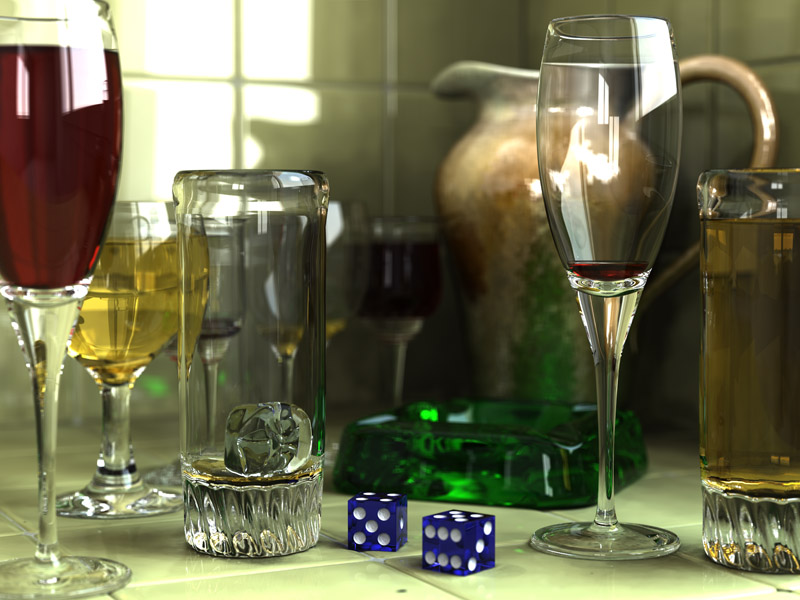
\includegraphics[width=14cm]{glasses.jpg}
\caption{Glasses - grafika wygenerowana przy użycie programy \emph{POV-Ray}, autor: Gilles Tran, źródło: http://www.oyonale.com/modeles.php?lang=en\&page=40}
\end{figure}

Metoda śledzenia promieni jest stosunkowo prostym algorytmem, który pozwala na generowanie bardzo złożonych i realistycznych grafik uwzględniających wiele zjawisk fizycznych. Wadą takiego rozwiązanie jest bardzo długi czas generowania obrazu, dlatego nie jest ono wykorzystywane w aplikacjach interaktywnych. Zamiast tego wykorzystuje się tzw. \emph{computer graphics pipeline} - skomplikowaną, wspieraną sprzętowo sekwencję kroków wykorzystywanych w bibliotekach graficznych takich jak \emph{OpenGL} (dokładny opis działania można znaleźć w \cite{gpipe}). Pozwala ona na szybkie renderowanie obiektów, jednak obrazy wygenerowane tą metodą nie będą już tak realistyczne - wiele pracy wkłada się w poprawienie ich jakości.

Podstawowym pytaniem, jakie jest stawiane w tej pracy, jest to, czy metoda śledzenia promieni ma szansę być wykorzystywana w aplikacjach interaktywnych tak, aby obliczenia związane z generowaniem obrazu były niewidoczne dla użytkownika? Jakie parametry sceny pozwalają na generowanie obrazu z zadowalającą prędkością? Czy zrównoleglenie obliczeń pozwoli zbliżyć się do minimalnego progu 24 klatek na sekundę tak, aby można było mówić o generowaniu obrazu w czasie rzeczywistym? W jaki sposób moglibyśmy przyspieszyć obliczenia?  Wiele z tych pytań pozostanie otwartych, jednak badania takie jak te są próbą znalezienia na nie odpowiedzi.


\section{Wykazu celów i zadań pracy}

Celem niniejszej pracy jest:
\begin{enumerate}
\item Dokonanie analizy problemu na podstawie zebranej literatury.
\item Określenie wymagań jakie powinien spełniać system.
\item Dobór narzędzi programistycznych w celu zaimplementowania systemu realizującego algorytm śledzenia promieni.
\item Zaprojektowanie systemu.
\item Implementacja systemu.
\item Przeprowadzenie badań nad algorytmem metody śledzenia promieni.
\item Omówienie rezultatów.
\item Zaproponowanie dodatkowych rozwiązań mających na celu przyspieszenie obliczeń.
\end{enumerate}

\section{Budowa pracy}

Niniejszy dokument składa się z ośmiu rozdziałów - ten, stanowiący wstęp, jest jednym z nich. W rozdziale drugim znajduje się dogłębna analiza problemu - zostały tam w sposób szczegółowy przedstawione wszystkie podejmowane zagadnienia. W rozdziale trzecim zostały zaproponowane technologie, które pozwolą na implementację programu mającego realizować rekursywną metodę śledzenia promieni z wykorzystaniem obliczeń równoległych. Na początku rozdziału czwartego zostały zdefiniowane wymagania i założenia, jakie powinien realizować program. Kolejne podrozdziały w sposób bardziej formalny i szczegółowy pokazują architekturę aplikacji. W rozdziale piątym zostały zawarte niektóre szczegóły implementacyjne gotowego już programu. Rozdział szósty opisuje, w jaki sposób program działa - przedstawiono tam podstawową instrukcję jego obsługi oraz budowę pliku wejściowego. Rozdział siódmy zawiera rezultaty przeprowadzonych testów, wraz z ich omówieniem. Znajdują tam się również przykładowe obrazy, jakie zostały wygenerowane przez działającą aplikację. W rozdziale ósmym znajduje się podsumowanie pracy wraz z propozycjami kierunku dalszych badań.

\chapter{Analiza problemu}
\section{Podstawowy algorytm śledzenia promieni}
\section{Równoległy algorytm śledzenia promieni}
\section{Wybór technologii}


\chapter{Projekt systemu}
W tym rozdziale przedstawiono projekt systemu, który ma zostać zaimplementowany na potrzeby tej pracy. Projektowany system powinien umożliwiać uruchomienie aplikacji na dowolnie dużym klastrze obliczeniowym składającym się z maszyn o różnej specyfikacji. Na komputerze, na którym aplikacja jest uruchamiana (a więc tym wykorzystywanym przez użytkownika) powinno uruchomić się okno dające podgląd na generowaną animację. Aplikacja powinna dawać możliwość załadowania pliku opisującego scenę, która następnie będzie rozesłana do wszystkich węzłów klastra. Opis działania klastra i planowanych klas programu (powiązania między nimi i rola w systemie) został umieszczony poniżej. 

\section{Projekt klastra}

\begin{figure}[h!]
\centering
  \caption{Schemat systemu}
  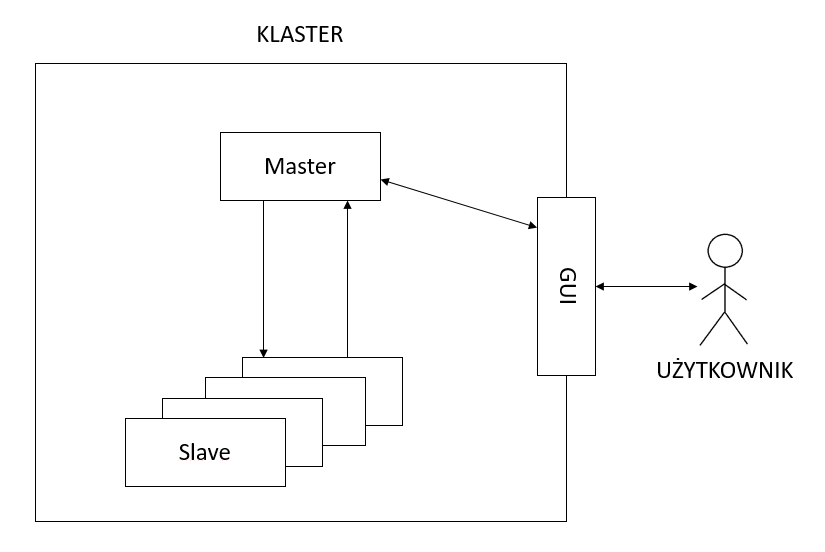
\includegraphics[width=10cm]{cluster.png}
\end{figure}

Na poniższym schemacie przedstawiono konceptualny schemat działania systemu. W założeniach, użytkownik ma komunikować się z klastrem poprzez graficzny interfejs użytkownika (zbudowany z wykorzystaniem biblioteki Qt), który udostępni mu podgląd dynamicznie budowanej animacji i wszelkich statystyk z nią związanych. Program master'a (a więc głównego węzła klastra) ma wykonywać się na tej samej maszynie, która udostępnia interfejs - główny proces zostanie podzielony na dwa wątki: jeden zajmujący się obsługą klastra (wątek master'a) i drugi związany z użytkownikiem (wątek GUI). Węzeł zarządzający komunikuje się z każdym z węzłów wykonawczych, zlecając im zadania i zbierając od nich wyniki. W chwili, w której zostanie wygenerowana cała klatka, master informuje wątek GUI, o tym że wygenerowany obraz jest gotowy do wyświetlenia. W poniższych punktach zostanie zaprezentowany proponowany algorytm zachowania węzłów.  
	
\subsection{Master}

Pierwszym i najważniejszym zadaniem węzła zarządzającego jest wczytanie pliku zawierającego definicję generowanego obrazu. Na podstawie pliku wejściowego ma on stworzyć scenę, kamerę, obiekty i światła. Następnie musi on rozesłać informacje na temat obiektów do wszystkich węzłów wykonawczych, tak aby każdy z nich posiadał tę samą definicję obrazu (broadcast). Gdy już każdy z węzłów zasygnalizuje gotowość, węzeł zarządzający rozsyła zadania policzenia danego wycinka obrazu do węzłów wykonawczych. Poniżej przedstawiono przykładowy pseudokod działania master'a. Warto zwrócić uwagę, że zadania umieszczane są w kolejce oczekującej - takie rozwiązanie powinno dawać lepsze rezultaty niż rozesłanie do węzłów wszystkich zadań od razu, ponieważ różne fragmenty obrazu mogą być generowane z różną prędkością. Mogłoby więc dochodzić do sytuacji, w której część węzłów zrealizowała już swoje zadania (a więc ich moc obliczeniowa nie jest wykorzystywana), a część (która dostała bardziej wymagające obliczenia) ciągle liczy.

\begin{algorithm}
\begin{algorithmic}
\State readFile()
\State sendScene()
\State sendCamera()
\\
\While{true}
\\
\State queue = splitImageToChunks()
\State //pending - liczba zleconych, niewykonanych zadań
\State pending = sendChunkToEveryNode()
\\
\While {pending $>$ 0}
\State msg = recvMessage()
\If {msg == EXIT} exit()
\ElsIf {msg = PIXELS}
	recvPixels()
	\If {queue is not empty}
		sendChunkToSlave()
	\Else
		pending--
	\EndIf
\EndIf
\EndWhile
\State informGUI()
\State updateCameraPos()
\EndWhile
\end{algorithmic}
\end{algorithm}


\subsection{Slave}

Nawiązując do poprzedniego punktu, pierwszą czynnością, którą powinien wykonać każdy ze slave'ów, jest odebranie definicji obiektów wykorzystywanych przy generowaniu sceny. Następnie w pętli, może on czekać na zadanie, realizować je (z wykorzystaniem klasy RayTracer) i odsyłać z powrotem do węzła zarządzającego.

\begin{algorithm}
\begin{algorithmic}
\State recvScene()
\State recvCamera()
\\
\While{true}
\State msg = recvMessage()
\If {msg == EXIT} exit()
\ElsIf {msg == CHUNK}
	recvChunk()
	pixels = recursiveRayTracer()
	sendPixels()
\ElsIf {msg == CAMERA}
	recvCamera() //aktualizacja pozycji kamery
\EndIf
\EndWhile
\end{algorithmic}
\end{algorithm}


\section{Projekt programu}

	\subsection{Diagram klas}
	\begin{figure}[H]
    \centering
              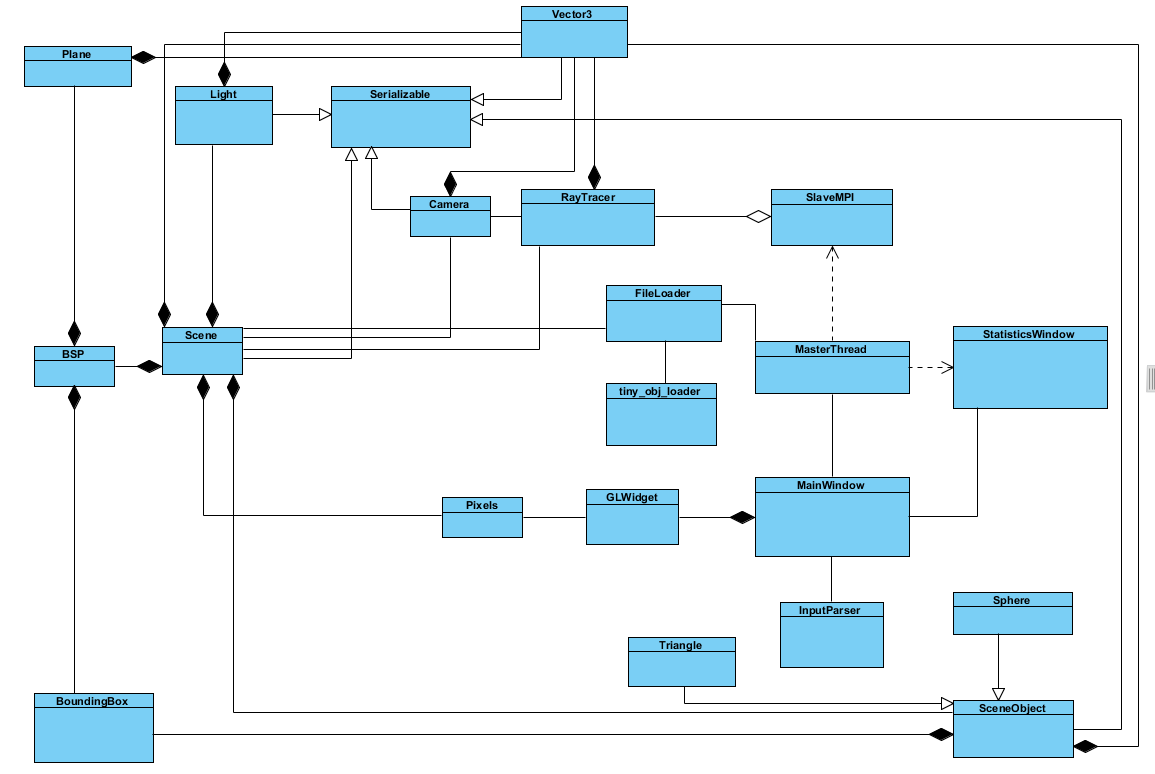
\includegraphics[angle=90,width=\textwidth,
                    height=0.8\textheight,
                   ]{classDiagram.PNG}
    \caption{Diagram klas}
    \label{fig:classDiagram}
	\end{figure}
	
	Powyżej przedstawiono uproszczony diagram klas. Opis poszczególnych z nich (wraz ze spisem atrybutów i metod) znajduje się w kolejnym podrozdziale.
	
\subsection{Opis klas}

\subsubsection{BoundingBox}


\footnotesize
\footnotesize
\begin{longtable}{|p{14cm}|}
	\caption{BoundingBox} \label{tab:BoundingBox} \\ \hline
	\multicolumn{1}{|c|}{BoundingBox} \\ \hline
    +minX : float \\
    +maxX : float \\
    +minY : float \\
    +maxY : float \\
    +minZ : float \\
    +maxZ : float \\ \hline
    +intersect(start: Vector3, dir: Vector3 \\ \hline
\end{longtable}
\normalsize

Klasa BoundingBox reprezentuje prostopadłościany, które w założeniu mają otaczać inne obiekty (bryła otaczająca). Ma ona umożliwić przyspieszenie badania przecięcia promieni z elementami sceny (stąd metoda intersect). W programie będzie wykorzystywana przez drzewo BSP (otoczenie całej sceny) i SceneObject. 


\subsubsection{BSP}

\footnotesize
\begin{longtable}{|p{14cm}|}
	\caption{BSP} \label{tab:BSP} \\ \hline
	\multicolumn{1}{|c|}{BSP} \\ \hline

    +tree : node* \\
    -polygons : SceneObject* \\
    -box : BoundingBox \\ \hline
    +build(root : node*, polygons : SceneObject*, depth : int) \\ 
	-getBestPlane(polygons : list$<$SceneObject*$>$) : Plane \\
	+getClosest(cross : Vector3, start : Vector3, dir : Vector3) : SceneObject* \\
	+isInShadow(cross : Vector3, dir : Vector3, light : Vector3) : bool \\
	-getBoundingBox(polygons : list$<$SceneObject*$>$) : BoundingBox \\
	-intersect(root : node*, cross : Vector3, start : Vector3, dir : Vector3) : SceneObject* \\
	-deleteTree(root : node*) : void \\
    \hline
\end{longtable}
\normalsize

\footnotesize
\begin{longtable}{|p{14cm}|}
    \caption{Node} \label{tab:Node} \\ \hline
    \multicolumn{1}{|c|}{Node} \\ \hline
    partitionPlane : Plane \\
    polygons : list$<$SceneObject*$>$ \\
    front : node*  \\
    back : node*  \\ \hline
\end{longtable}
\normalsize

Klasa BSP implementuje drzewo opisane w rozdziale (!RODZIAŁ!). Poza metodami związanymi z budową drzewa, zawiera ona metody analogiczne do Klasy Scene (z tą różnicą, że metody Scene wykorzystują przegląd zupełny obiektów) umożliwiające przeglądanie sceny w poszukiwaniu przeciętych obiektów i badania, czy dany punkt znajduje się w cieniu. Drzewo BSP jest składową klasy Scene, która wywołuje jego metody (jeżeli jest ustawiona flaga mówiąca o wykrzystaniu drzewa).

Podstawowym elementem drzewa jest struktura Node, która zawiera pola takie jak płaszczyzna podziału, wskaźniki na kolejne wierzchołki drzewa (reprezentujące przestrzeń przed i za płaszczyzną) i listę obiektów należących do danego wierzchołka. Obiekt może należeć do wierzchołka np. w sytuacji gdy wierzchołek jest liściem lub obiekt leży na płaszczyźnie podziału. Klasa BSP zostanie dokładniej opisana w rozdziale 6.

\subsubsection{Camera}

\footnotesize
\begin{longtable}{|p{14cm}|}
    \caption{Camera} \label{tab:Camera} \\ \hline
    \multicolumn{1}{|c|}{Camera} \\ \hline
    +zNear : float \\
    +zFar : float \\
    +pixWidth : int \\
    +pixHeight : int \\
    +povy : float \\
    +aspect : float \\
    +worldWidth : float \\
    +worldHeight : float \\
    +R : float \\
    +ver : float \\
    +hor : float \\
    +instance : Camera* \\ 
    +eye : Vector3<float>* \\
    +look : Vector3<float>* \\
    +up : Vector3<float>* \\
    +lookAt : Vector3<float>* \\
    \hline
    +setUp(pixWidth : int, pixHeight : int) : void \\
    +getInstance() : Camera * \\
    +getWorldPosOfPixel(x : int, y : int) : Vector3<float> \\
    +rotate() : void \\
    \hline
\end{longtable}
\normalsize

Podobnie jak obiekt klasy Scene, obiekt klasy Camera jest zbudowany według wzorca Singleton (może istnieć tylko jeden obiekt takiej klasy). Klasa ta definiuje obiekt wirtualnej kamery, którą możemy umiejscowić w dowolnym miejscu i (z jej perspektywy) obserwować dowolny skrawek sceny. To ona zapewnia definicję rzutni i pozwala na translację współrzędnych świata (okno obserwatora) na współrzędne urządzenia (piksele ekranu).

\subsubsection{GLwidget}

\footnotesize
\begin{longtable}{|p{14cm}|}
    \caption{GLwidget} \label{tab:GLwidget} \\ \hline
    \multicolumn{1}{|c|}{GLwidget} \\ \hline
    scene : Scene*  \\ \hline
    initializeGL() : void \\ 
    resizeGL(int w, int h) : void \\
    paintGL() : void \\ \hline
\end{longtable}
\normalsize

Widgety są składowymi elementami graficznego interfejsu użytkownika i nie wszystkie z nich muszą być reprezentowane poprzez obiekty. Klasa GLwidget odpowiada za prezentowanie kolejnych klatek użytkownikowi. W przypadku kiedy główne okno aplikacji (MainWindow, ,,rodzic'' GLwidget) otrzyma informacje o wygenerowaniu kolejnej klatki od MasterThread wywołuje odpowiednią metodę GLwidget - GLwidget odwołuje się do Klasy Scene, od której otrzymuje tablicę pikseli (Pixels) do wyświetlenia. 

\subsubsection{FileLoader}

\footnotesize
\begin{longtable}{|p{14cm}|}
    \caption{FileLoader} \label{tab:FileLoader} \\ \hline
    \multicolumn{1}{|c|}{FileLoader} \\ \hline
    -readCameraSettings(line : char const*) : bool \\
    -readSceneSettings(line : char const*) : bool \\
    -readSphere(line : char const*) : bool \\
    -readLight(line : char const*) : bool \\
    -readTriangle(line : char const*) : bool \\
    -readObj(line : char const*) : bool \\
	+ReadFile(fname : char const*) : bool \\ \hline
\end{longtable}
\normalsize

FileLoader jest klasą odpowiedzialną za wczytanie definicji sceny z pliku (stąd powiązania z klasami Scene i Camera). Jest ona wykorzystywana przez klasę MasterThread. Klasa korzysta z biblioteki tinyobjloader, dzięki której możliwe jest wczytywanie modeli zapisanych w formacie ,,obj''. Bibliotekę można znaleźć pod adresem https://github.com/syoyo/tinyobjloader. Jest ona udostępniona na licencji MIT.

\subsubsection{InputParser}

\footnotesize
\begin{longtable}{|p{14cm}|}
    \caption{InputParser} \label{tab:InputParser} \\ \hline
    \multicolumn{1}{|c|}{InputParser} \\ \hline
    tokens : vector$<$string$>$  \\ \hline
    +getCmdOption(option : string const) : string const) \\
    +cmdOptionExists(option : string const) : bool \\ \hline
\end{longtable}
\normalsize

Klasa InputParser jest prostą klasą pozwalająca na obróbkę danych wejściowych (dokładniej opisane w rozdziale !WSTAW RODZIAŁ!). Klasa MainWindow, która w założeniach ma tworzyć wątek MasterThread, wykorzystuje ją do przekazania mu parametrów.

\subsubsection{Light}

\footnotesize
\begin{longtable}{|p{14cm}|}
    \caption{Light} \label{tab:Light} \\ \hline
    \multicolumn{1}{|c|}{Light} \\ \hline
    +pos : Vector3* \\ 
    +amb : Vector3* \\
    +dif : Vector3* \\
    +spec : Vector3* \\
    \hline
	+serialize(bytes : vector$<$char$>$*) : void \\ 
	+deserialize(bytes : vector$<$char$>$ const) : void \\
	+getType() : char \\
	\hline
\end{longtable}
\normalsize

Klasa Light określa obiekty światła. Więcej o świetle i jego znaczeniu na scenie można przeczytać w rozdziale !ROZDZIAŁ!.

\subsubsection{MainWindow}

\footnotesize
\begin{longtable}{|p{14cm}|}
    \caption{MainWindow} \label{tab:MainWindow} \\ \hline
    \multicolumn{1}{|c|}{MainWindow} \\ \hline
    ui : MainWindow* \\
    statisticWindow : StatisticsWindow* \\
    masterThread : MasterThread* \ \
    statusLabel : QLabel* \\ \hline
    createMaster() \\
    ShowStats() \\
    setSpeed(double time) \\
    on\_actionStatistics\_triggered() \\
    onQuit(); \\ \hline
\end{longtable}
\normalsize

Klasa MainWindow reprezentuje główne okno aplikacji. Ze względów projektowych jest ona odpowiedzialna za tworzenie obiektu MasterThread (ma to związek z mechanizmem przypisania sygnałów do slotów - mechanizm komunikacji międzywątkowej w Qt) jak i potrzebie komunikacji między jedną i drugą klasą. Klasa MainWindow (wraz z GLwidget i StatisticWidnow) reprezentuje warstwę prezentacji tworzonej aplikacji.

\subsubsection{MasterThread}

\footnotesize
\begin{longtable}{|p{14cm}|}
    \caption{MasterThread} \label{tab:MasterThread} \\ \hline
    \multicolumn{1}{|c|}{MasterThread} \\ \hline
    isAlive : bool \\
    camera : Camera* \\
    scene : Scene* \\
    processSpeed : double** \\
    worldSize : int \\
    status : MPI\_Status \\
    names : vector$<$string$>$ \\
    pending : int \\
    numChunks : int \\
    queue : queue$<$Chunk$>$ \\
    test : int \\
    \hline
	run() \\
	splitToChunks(int num) \\
	clearQueue(queue$<$Chunk$>$ q) \\
    sendCameraBcast() \\
    sendCameraPointToPoint() \\
    sendScene() \\
    sendDepth(int depth) \\
    sendNextChunk(int dest) \\
    sendExitSignal() \\
    recvPixels(MPI\_Status stat) : int \\
    recvMessage() : int \\
    finishPending() \\
    updateProcessSpeed() \\
    waitUntillRdy() \\
    printResult(double spf, double bsp) \\
    getNames() \\
    emitNames() \\
	\hline
\end{longtable}
\normalsize

Klasa MasterThread jest główną klasa aplikacji, której obiekt tworzony jest w tym samym procesie co obiekt MainWindow, jednak działa w osobnym wątku. Takie rozwiązanie pozwala zachować responsywność aplikacji. Wątek okna głównego jest odpowiedzialny za przetwarzanie zdarzeń wygenerowanych przez użytkownika czy program, a wątek MasterThread, niezależnie od niego, zajmuje się w tym czasie generowaniem kolejnej klatki animacji. Rozdzielamy w ten sposób warstwę prezentacji od warstwy biznesowej tworząc tym samym aplikację przyjaźniejszą użytkownikowi.

Głównym zadaniem MasterThread jest zarządzanie węzłami wykonawczymi (sam stanowi on serce węzła nadzorującego). Posiada on szereg metod umożliwiających komunikację z innymi procesami tworzącymi aplikację. Ma on dostęp do lokalnych kopii obiektów Scene i Camera, ponieważ musi je rozesłać po klastrze i mieć możliwość modyfikacji ich parametrów (przesunięcie kamery co klatkę, aktualizacja obiektu Pixels). Więcej o zadaniach i sposobie działania MasterThread można przeczytać (!rodział z wyżej!, !rodział z implementacji!).

\footnotesize
\begin{longtable}{|p{14cm}|}
    \caption{Chunk} \label{tab:Chunk} \\ \hline
    \multicolumn{1}{|c|}{Chunk} \\ \hline
    startx : int \\
    stopx : int \\
    starty : int \\
    stopy : int \\
    \hline
\end{longtable}
\normalsize

Chunk jest prostą strukturą wykorzystywaną w komunikacji Master/Slave (MasterThread, SlaveMPI). Zawiera on w sobie informacje o tym, jaki wycinek obrazu powinien być wyznaczany przez dany węzeł wykonawczy.


\subsubsection{Pixels}

\footnotesize
\begin{longtable}{|p{14cm}|}
    \caption{Pixels} \label{tab:Pixels} \\ \hline
    \multicolumn{1}{|c|}{Pixels} \\ \hline
    +data : unsigned char* \\
    +x : int \\
    +y : int \\ 
    +startx : int \\
    +starty : int \\
    \hline
	+serialize(bytes : vector$<$char$>$*) : void \\
	+deserialize(bytes : vector$<$char$>$ const) : void \\
	+getType() : char \\
	+setStartXY(x : int, y : int) : void \\
	+setPixel(posX : int, posY : int, vec : Vector3) : void \\
	\hline
\end{longtable}
\normalsize

Klasa Pixels przechowuje tablice pikseli w formie ciągu bajtów unsigned char* (taka reprezentacja jest wykorzystywana przez funkcje rysujące, które zapewniają przyspieszenie sprzętowe). Pozwala ona stworzyć wygodny interfejs czytania i pisania do tablicy. 

\subsubsection{Plane}

\footnotesize
\begin{longtable}{|p{14cm}|}
    \caption{Plane} \label{tab:Plane} \\ \hline
    \multicolumn{1}{|c|}{Plane} \\ \hline
    +a : float \\ 
    +b : float \\
    +c : float \\
    +d : float \\
    \hline
	+classifyObject(obj : SceneObject*) : int \\
	+classifyPoint(point : Vector3*) : int \\
	+getDistToPoint(point : Vector3*) : float \\
	+rayIntersectPlane(start : Vector3, dir : Vector3) : bool \\
	+getNormal() : Vector3 \\
	+isValid() : bool \\
	\hline
\end{longtable}
\normalsize

Klasa reprezentuje obiekty płaszczyzn, wykorzystywane przy podziale podprzestrzeni przez drzewo BSP. Zawiera metody pozwalające określić, po której stronie płaszczyzny znajduje się dany obiekt.

\subsubsection{RayTracer}

\footnotesize
\begin{longtable}{|p{14cm}|}
    \caption{RayTracer} \label{tab:RayTracer} \\ \hline
    \multicolumn{1}{|c|}{RayTracer} \\ \hline
    +camera : Camera* \\
    +scene : Scene* \\ \hline
	+basicRayTracer() : void \\
	+recursiveRayTracer(depth : int) : void \\
	+getColorRecursive(start : Vector3, dir : Vector3, depth : int) : Vector3 \\
	\hline
\end{longtable}
\normalsize

Klasa RayTracer zawiera w sobie zestaw metod, które pozwalają na realizację algorytmu śledzenia promieni. W tym celu odwołuje się ona do pól klas Scene i Camera. Każdy obiekt SlaveMPI (zawierający w sobie algorytm działający na węzłach wykonawczych) tworzy własny obiekt RayTracer'a. Klasa ta zostanie dokładniej opisana w rozdziale 6.

\subsubsection{Scene}

\footnotesize
\begin{longtable}{|p{14cm}|}
    \caption{Scene} \label{tab:Scene} \\ \hline
    \multicolumn{1}{|c|}{Scene} \\ \hline
    +numOfLights : int \\
    +numOfObjects : int \\
    +useShadows : bool \\
    +useBSP : bool \\
    +instance : Scene* \\
    +lights : Light** \\
    +sceneObjects : SceneObject** \\
    +pixels : Pixels* \\
    +backgroundColor : Vector3* \\
    +globalAmbient : Vector3* \\
    +bsp : BSP* \\
    \hline
	+getInstance() : Scene * \\
	+buildBSP(depth : int) : void \\
	+addObject(sceneObject : SceneObject*) : void \\
	+addLight(light : Light*) : void \\
	+setUpPixels(x : int, y : int) : void \\
	+getClosest(cross : Vector3, start : Vector3, dir : Vector3) : SceneObject * \\
	+isInShadow(cross : Vector3, dir : Vector3, lightPos : Vector3) : bool \\
	+setPixelColor(x : int, y : int, color : Vector3) : void \\
	+serialize(bytes : vector$<$char$>$*) : void \\
	+deserialize(bytes : vector$<$char$>$ const) : void \\
	+getType() : char \\
	\hline
\end{longtable}
\normalsize

Obiekt klasy Scene zawiera definicję całej sceny. Jest on napisany według wzorca Singleton (może istnieć tylko jeden obiekt takiej klasy). Wywołując statyczną metodę getInstance() otrzymamy na niego wskaźnik. Obiekt Scene jest jednym z częściej wykorzystywanych obiektów, gdyż jest centralnym elementem aplikacji - zawiera pola istotne dla wielu klas. W związku z tym udostępnia on interfejs pozwalający na pobieranie interesujących daną klasę danych (np. metoda isInShadow, która bada czy dany punkt znajduje się w cieniu. Klasa, zgodnie z flagą useBSP, dokonuje przeglądu zupełnego lub wykorzystuje drzewo).

\subsubsection{SceneObject}

\footnotesize
\begin{longtable}{|p{14cm}|}
    \caption{SceneObject} \label{tab:SceneObject} \\ \hline
    \multicolumn{1}{|c|}{SceneObject} \\ \hline
    \#specShin : float \\
    \#transparency : float \\
    \#mirror : float \\
    \#local : float \\
    \#density : float \\
    \#amb : Vector3* \\
    \#dif : Vector3* \\
    \#spec : Vector3* \\
    \hline
	+getLocalColor(normal : Vector3, cross : Vector3, observation : Vector3) : Vector3 \\
	+trace(cross : Vector3, start : Vector3, dir : Vector3, dist : float) : bool \\
	+getNormalVector(cross : Vector3) : Vector3 \\
	+getBoundingBox() : BoundingBox \\
	\hline
\end{longtable}
\normalsize

SceneObject jest wirtualną klasą po której powinny dziedziczyć wszystkie obiekty sceny. Pozwala ona na wykorzystywanie wielopostaciowości (widoczne np. w klasie Scene), wymuszając na klasach potomnych implementacje metod pozwalających określić przecięcie z promieniem (trace()), oblicznie wektora normalnego w punkcie (getNormalVector()), czy pobranie koloru w punkcie (getLocalColor())

\subsubsection{Serializable}

\footnotesize
\begin{longtable}{|p{14cm}|}
    \caption{Serializable} \label{tab:Serializable} \\ \hline
    \multicolumn{1}{|c|}{Serializable} \\ \hline
    +serializedSize : int \\ \hline
	+serialize(bytes : vector$<$char$>$*) : void \\ 
	+deserialize(bytes : vector$<$char$>$ const) : void \\
	+getType() : char \\
	\hline
\end{longtable}
\normalsize

Klasa Serializable jest właściwie Interfejsem - dziedziczą po niej wszystkie klasy, które muszą mieć możliwość serializacji (zamiana obiektu na ciąg bajtów) w związku z potrzebą wysłania ich do innych węzłów klastra. Bardziej szczegółowe informacje o serialializacji można znaleźć w rodziale 6.

\subsubsection{SlaveMPI}

\footnotesize
\begin{longtable}{|p{14cm}|}
    \caption{SlaveMPI} \label{tab:SlaveMPI} \\ \hline
    \multicolumn{1}{|c|}{SlaveMPI} \\ \hline
    +x : int \\ 
	+y : int \\
	+depth : int \\
	+status : MPI\_Status \\
	+pixels : Vector3*** \\
	+camera : Camera* \\
	+scene : Scene* \\ \hline
	+exec() : int \\
	+recvCameraBcast() : void \\
	+recvCameraPointToPoint() : void \\
	+recvScene() : void \\
	+recvDepth() : void \\
	+recvChunk() : void \\
	+recvMessage() : int \\
	+sendPixels() : void \\
	+sendName() : void \\
	+sendRdy() : void \\
	\hline
\end{longtable}
\normalsize

SlaveMPI jest klasą analogiczną do klasy MasterThraed, jednak jej obiekt jest tworzony na każdym węźle wykonawczym. Zawiera ona w sobie metody implementujące mechanizmy komunikacji z resztą węzłów i takie pozwalające na wykonywanie zadań zleconych przez mastera. Metoda exec() implementuje algorytm opisany w rozdziale (!wstaw rozdział!) - główną pętlę programu węzłów wykonawczych. Więcej o implementacji można znaleźć w rozdziale 6.

\subsubsection{StatisticsWindow}

\footnotesize
\begin{longtable}{|p{14cm}|}
    \caption{StatisticsWindow} \label{tab:StatisticsWindow} \\ \hline
    \multicolumn{1}{|c|}{StatisticsWindow} \\ \hline
    Ui::StatisticsWindow *ui; \\
    int worldSize; \\
    \hline
	resizeEvent(QResizeEvent *event) : void \\
    setTime(double time) : void  \\
    setChunks(int i) : void \\
    setXY(int x, int y) : void \\
    setObj(int i) : void \\
    setLights(int i) : void  \\
    setProccessName(int num, QString str) : void \\
    setProccessSpeed(double **speed) : void \\
    setUpList() : void \\
    \hline
\end{longtable}
\normalsize

StatisticWindow jest oknem, które (jak sama nazwa wskazuje) ma prezentować statystki dotyczące programu - czas generowania jednej klatki, średni czas pracy danego węzła, liczbę obiektów na scenie itd.

\subsubsection{Sphere}

\footnotesize
\begin{longtable}{|p{14cm}|}
    \caption{Sphere} \label{tab:Sphere} \\ \hline
    \multicolumn{1}{|c|}{Sphere} \\ \hline
    +radius : float \\
    +pos : Vector3* \\
    \hline
\end{longtable}
\normalsize

Klasa Sphere jest klasą reprezentującą sferę. Dziedziczy ona po SceneObject, a więc implementuje metody specyficzne dla tego typu obiektu (np. badanie przecięcia z promieniem).

\subsubsection{Triangle}

\footnotesize
\begin{longtable}{|p{14cm}|}
    \caption{Triangle} \label{tab:Triangle} \\ \hline
    \multicolumn{1}{|c|}{Triangle} \\ \hline
    +pointA : Vector3* \\
    +pointB : Vector3* \\
    +pointC : Vector3* \\
    +normalA : Vector3* \\
    +normalB : Vector3* \\
    +normalC : Vector3* \\
    \hline
	+split(plane : Plane, front : list$<$Triangle*$>$, back : list$<$Triangle*$>$) : void \\ 
	+getPointbyNum(a : int) : Vector3 * \\
	+getPlanes() : list$<$Plane$>$ \\
	+getPerpendicularPlane(i : int) : Plane \\
	+getPlane() : Plane \\
	+Area(a : Vector3, b : Vector3) : float \\
	+getBoundingBox() : BoundingBox \\
	\hline
\end{longtable}
\normalsize

Triangle jest klasą reprezentującą obiekty trójkąta. Triangle podobnie jak Sphere dziedziczy po SceneObject i implementuje metody specyficzne dla tego typu obiektu.

\subsubsection{Vector3}

\footnotesize
\begin{longtable}{|p{14cm}|}
    \caption{Vector3} \label{tab:Vector3} \\ \hline
    \multicolumn{1}{|c|}{Vector3} \\ \hline
    +x : type \\
    +y : type \\
    +z : type \\
     \hline
	+normalize() : Vector3 \\ 
	+scalarProduct(v : Vector3) : float \\
	+vectorProduct(v : Vector3) : Vector3 \\
	+rotateX(alpha : float) : void \\
	+rotateY(alpha : float) : void \\
	+rotateZ(alpha : float) : void \\
	+distanceFrom(v : Vector3) : float \\
	+powDistanceFrom(v : Vector3) : float \\
	+reflect(n : Vector3) : Vector3 \\
	+refract(normalVector : Vector3, a : float, b : float) : Vector3 \\
	+isZeroVector() : bool \\
	+length() : float \\
	\hline
\end{longtable}
\normalsize

Klasa Vector3 jest klasą pozwalającą definiować obiekty takie jak punkt, czy wektor w przestrzeni 3D. Zapewnia ona szereg metod implementujących różne operacje matematyczne na tego typu obiektach. Poza implementacją wszystkich metod zawartych w tabeli wyżej, zostanie również przeciążona część operatorów arytmetycznych - ułatwi to korzystanie z klasy.


\chapter{Opis wybranych technologii}
	\section{C++}
	\section{QT}
	\section{Standard MPI}

\chapter{Implementacja}
\section{Szczegółowy opis wybranych fragmentów kodu}
	\subsection{RayTracer}

Klasa \emph{RayTracer} implementuje zestaw metod realizujących algorytm śledzenia promieni. Korzysta ona z interfejsu udostępnianego przez klasy takie jak \emph{Scene} czy \emph{Camera}, aby generować kolejne promienie do wysłania. Poniżej zostały omówione dwa najważniejsze fragmenty kodu zawarte w tej klasie:
	
\begin{lstlisting}[caption={Fragment klasy \emph{RayTracer}}]

void RayTracer::recursiveRayTracer(int depth) {

Vector3<float> worldPosOfPixel;
Vector3<float> directionVector;

for(int i = 0; i < scene->getWidth(); i++) {
    for(int j = 0; j < scene->getHeight(); j++) {
        worldPosOfPixel = camera->getWorldPosOfPixel(i + scene->getStartX(),j + scene->getStartY());
        directionVector = worldPosOfPixel - *camera->getEye();
        directionVector.normalize();
        scene->setPixelColor(i, j, getColorRecursive(worldPosOfPixel, directionVector, depth));
    }
}
}
\end{lstlisting}	

Powyższy fragment kodu implementuje algorytm, który można znaleźć w rozdziale !TU WSTAW RODZIAŁ!. Dla każdego piksela sceny zostaje wygenerowany promień pierwotny (\emph{directionVector}), który następnie jest wysyłany w scenę - funkcja \emph{getColorRecursive} (opisana niżej) zwraca kolor, jaki należy przypisać danemu punktowi ekranu. Każdy z węzłów wykonawczych posiada swój egzemplarz obiektu klasy \emph{Scene} (wykorzystywany w powyższym kodzie) zmodyfikowany w taki sposób, aby przechowywał on jedynie fragment obrazu (\emph{Pixels)} - początek wycinka jest określany zmiennymi \emph{startX} i \emph{startY}, a zmodyfikowane wymiary obrazu pozwalają określić jego koniec. Więcej o komunikacji Master/Slave można przeczytać w rozdziałach !TU WSTAW RODZIAŁY!. 

\begin{lstlisting}[caption={Fragment klasy \emph{RayTracer}}]

Vector3<float> RayTracer::getColorRecursive(Vector3<float> startPoint, Vector3<float> directionVector, int depth)
{

SceneObject* sceneObject;
Vector3<float> crossPoint;
Vector3<float> reflectedRay;
Vector3<float> localColor;
Vector3<float> reflectedColor;

//refraction
Vector3<float> transparencyColor;
Vector3<float> transparencyRay;

if (depth == 0)
    return Vector3<float>();

depth--;

sceneObject = scene->getClosest(crossPoint, startPoint, directionVector);

if (sceneObject == nullptr)
    return Vector3<float>(*scene->backgroundColor);

Vector3<float> normalVector = sceneObject->getNormalVector(crossPoint);
Vector3<float> observationVector = directionVector*-1;


if (observationVector.scalarProduct(normalVector) < 0) {
    normalVector = normalVector*-1;
}

if(sceneObject->getTransparency()>0) {
    transparencyRay = directionVector.refract(normalVector, sceneObject->getDensity(), 1);
    transparencyColor = getColorRecursive(crossPoint, transparencyRay, depth);
}

if (sceneObject->getLocal()>0) {
    localColor.setValues(sceneObject->getLocalColor(normalVector, crossPoint, observationVector));
}

if (sceneObject->getMirror()>0) {
    reflectedRay = directionVector.reflect(normalVector);
    reflectedColor = getColorRecursive(crossPoint, reflectedRay, depth);
}

return localColor*sceneObject->getLocal() + reflectedColor*sceneObject->getMirror() + transparencyColor*sceneObject->getTransparency();

}

\end{lstlisting}
	
Powyższa funkcja jest rekurencyjnie wywoływaną metodą pozwalającą określić ostateczny kolor piksela, z którego został wysłany promień pierwotny (wysłanie promienia pierwotnego następuje w funkcji \emph{recursiveRayTracer}). Przyjmuje ona promień (w postaci punktu początkowego i wektora kierunku) oraz zmienną określającą głębokość drzewa - jest ona dekrementowana z każdym kolejnym rekurencyjnym wywołaniem funkcji, a kiedy osiągnie zero, rekurencja jest przerywana. Pierwszym krokiem algorytmu jest stwierdzenie, czy promień przeciął się z jakimś obiektem (jest tutaj wykorzystywany albo przegląd zupełny, albo drzewo BSP). Jeżeli nie, to ostateczny kolor piksela (lub jego składowa na danym poziomie drzewa rekurencji) przyjmuje wartość koloru tła. Jeżeli tak, to algorytm wybiera obiekt będący najbliżej początku promienia (obiekt widoczny z perspektywy tego punktu) i (w zależności od modelu \emph{Phonga} i parametrów powierzchni omówionych w rozdziałach !TU WSTAW ROZDZIAŁ!) ustala lokalną barwę obiektu oraz wysyła dwa kolejne promienie mające wpływ na barwę ostateczną - promień odbity od powierzchni i promień przez nią przechodzący (jest tutaj uwzględnianie złamanie światła).
Ostateczny kolor piksela jest sumą kolorów lokalnych osiągniętych przez wszystkie promienie powstałe w wyniku wysłania promienia pierwotnego.	Niezrozumiały może wydawać się następujący fragment:

\begin{lstlisting}[caption={}]
if (observationVector.scalarProduct(normalVector) < 0) {
    normalVector = normalVector*-1;
}
\end{lstlisting}

Biorąc pod uwagę, że kierunek wektora normalnego ma wpływ na otrzymany kolor lokalny powierzchni (jeżeli jego kierunek jest niezgodny z kierunkiem światła to znaczy, że powierzchnia nie jest oświetlona) należy go odwrócić tak, aby był on zgodny z kierunkiem obserwacji - np. w sytuacji, w której obserwator znajdowałby się w kuli (wraz ze światłem oświetlającym scenę), a wektor normalny do powierzchni kuli skierowany byłby na zewnątrz, oświetlenie i tak nie miałoby na nią wpływu.

\subsection{BSP}

W tym punkcie zostanie przedstawione w jaki sposób zaimplementowano budowę drzewa BSP oraz jego przeglądanie.

\begin{lstlisting}[caption={Fragment klasy \emph{BSP} - budowa drzewa}]

root->partitionPlane = getBestPlane(polygons);
while(!polygons.empty()) {
    object = polygons.back();
    polygons.pop_back();
    result = root->partitionPlane.classifyObject(object);
    switch (result) {
        case FRONT:
            frontList.push_back(object);
        break;

        case BACK:
            backList.push_back(object);
        break;

        case COINCIDENT:
            backList.push_back(object);
            frontList.push_back(object);
        break;

        case SPANNING: {
            if (object->getType() == 's') {
                root->polygons.push_back(object);
            } else {
                Triangle *triangle = static_cast<Triangle*>(object);
                std::list<Triangle*> tempFrontList, tempBackList;
                triangle->split(root->partitionPlane, tempFrontList, tempBackList);
                while (!tempBackList.empty()) {
                    backList.push_back(tempBackList.back());
                    tempBackList.pop_back();
                }
                while (!tempFrontList.empty()) {
                    frontList.push_back(tempFrontList.back());
                    tempFrontList.pop_back();
            }
            }
        }
        break;

        default:
            break;
        }
    }
\end{lstlisting}

Powyższy fragment jest fragmentem kodu funkcji budującej drzewo, który nie został do końca uwzględniony w rozdziale (!TU WSTAW ROZDZIAŁ Z PSEUDOKODEM!). Pierwszym krokiem każdej kolejnej rekurencji budowy drzewa jest ustalenie płaszczyzny podziału - brane są pod uwagę wszystkie te, które są wyznaczane przez trójkąty zawarte w danym wierzchołku i te, które są do tych trójkątów prostopadłe (styczne z krawędziami). Poprzez najlepszą płaszczyznę rozumie się taką, która dzieli trójkąty na równe ilościowo grupy. Następnie w pętli algorytm sprawdza, po której stronie wybranej płaszczyzny znajduje się dany obiekt z listy - w zależności od sytuacji trafia on do listy, która zostanie przekazana kolejnym dzieciom (,,przedniemu'' i ,,tylnemu''). W przypadku, gdy trójkąt leży na płaszczyźnie podziału, jest on umieszczany w obu listach, z kolei jeżeli płaszczyzna go przecina, to jest on dzielony na dwa (w sytuacji powstania trójkąta i czworokąta, czworokąt jest dzielony na dwa trójkąty) - każda z połówek trafi do odpowiedniego ,,dziecka''. 	Program uwzględnia sfery przechowywane w postaci równania (a więc prosty podział takiego obiektu nie jest możliwy). W momencie, w którym płaszczyzna przetnie sferę, trafia ona tylko do listy obiektów rozpatrywanego wierzchołka. Zaimplementowanie sfer wymagało takiej niekonwencjonalnej modyfikacji algorytmu, która będzie miała wpływ na sposób przeglądania drzewa. Rekurencja kończy się, kiedy zostanie osiągnięta maksymalna głębokość drzewa (określana przez parametr przekazywany do funkcji przy pierwszym wywołaniu), lub w sytuacji, w której dalszy podział jest niemożliwy. Wtedy wierzchołek jest zamieniany w liść (wskaźniki na potomstwo są puste), a wejściowa lista obiektów zostaje do niego przypisana. Nie biorąc pod uwagę sfer wszystkie wierzchołki niebędące liśćmi są puste.

\begin{lstlisting}[caption={Fragment klasy \emph{BSP} - przeglądanie drzewa}]

SceneObject *BSP::intersect(BSP::node *root, Vector3<float> &crossPoint, Vector3<float> &startingPoint, Vector3<float> &directionVector) {

if (root->back == nullptr && root->front == nullptr) {
    return getClosestInNode(root->polygons, crossPoint, startingPoint, directionVector);
}

SceneObject *thisNodeHit = nullptr;
Vector3<float> tempCross;

if(!root->polygons.empty()) {
    thisNodeHit = getClosestInNode(root->polygons, tempCross, startingPoint, directionVector);
}

node *near;
node *far;
SceneObject *hit = nullptr;;


switch (root->partitionPlane.classifyPoint(&startingPoint)) {
    case FRONT:
        near = root->front;
        far = root->back;
    break;

    case BACK:
        near = root->back;
        far = root->front;
    break;

    case COINCIDENT: {

        Vector3<float> point = startingPoint + directionVector;
        if (root->partitionPlane.classifyPoint(&point) == FRONT) {
            near = root->front;
            far = root->back;
        }
        else {
            near = root->back;
            far = root->front;
        }
    }
    break;

    default:
        return nullptr;
        break;
}

hit = intersect(near, crossPoint, startingPoint, directionVector);

if (hit == nullptr && root->partitionPlane.rayIntersectPlane(startingPoint,directionVector)) {
    hit = intersect(far, crossPoint, startingPoint, directionVector);
}

if (thisNodeHit != nullptr) {
    if (hit != nullptr) {
        if (tempCross.distanceFrom(startingPoint) < crossPoint.distanceFrom(startingPoint)) {
            hit = thisNodeHit;
            crossPoint = tempCross;
        }
    }
    else {
        hit = thisNodeHit;
        crossPoint = tempCross;
    }
}
return hit;
}

\end{lstlisting}

Powyżej przedstawiono rekurencyjny algorytm przeszukiwania drzewa. Funkcja ta przyjmuje wskaźnik na sprawdzany wierzchołek drzewa i promień, a zwraca wskaźnik na znaleziony obiekt i punkt przecięcia (zmienna \emph{crossPoint} widoczna w liście parametrów).

Pierwszym krokiem algorytmu jest sprawdzenie, czy dany wierzchołek jest liściem. Jeżeli tak, to zostaje przeprowadzony test przecięcia na każdym obiekcie znajdującym się w wierzchołku - wybieramy najbliższy trafiony i zwracamy go do funkcji wywołującej. Następnie należy sprawdzić, czy dany wierzchołek rzeczywiście jest pusty (komplikacje spowodowane nietypowym obiektem nie będącym wielokątem - sferą). Jeżeli nie jest, to ponownie zostaną przeprowadzone testy przecięć dla każdego obiektu znajdującego się w wierzchołku - znaleziony obiekt przechowujemy w zmiennej \emph{thisNodeHit}.

Następnie, w zależności od tego, po której części płaszczyzny znajduje się punkt początkowy promienia, zostają ustawione zmienne ,,near'' (połowa, w której znajduje się punkt początkowy) i ,,far'' (alternatywa). W przypadku, w którym punkt startowy zawiera się w płaszczyźnie dzielącej, sprawdzamy, czy wektor kierunku nie jest równoległy do płaszczyzny - jeżeli jest ,,near'' i ,,far'' nie ma znaczenia; jeżeli nie jest, to jako ,,near'' wybieramy tę połowę wskazywaną przez wektor.

Kolejnym krokiem jest rekurencyjne wywołanie tej funkcji dla potomka ,,near''. Jeżeli nie zwróci ona żadnego obiektu, a promień przecina płaszczyznę dzielącą to rozwiązanie może znajdować się jeszcze w drugim potomku (,,far''). Ostatni fragment kodu sprawdza, czy jeżeli znaleziono obiekt w danym węźle i obiekt w jednym z dzieci, to który z nich jest bliżej - ten zostanie zwrócony jako wynik.

\subsection{MasterThread}
	
	
\begin{lstlisting}[caption={Fragment klasy \emph{MasterThread}}]

void MasterThread::run() {

while (true) {

    splitToChunks(numChunks);

    pending = 0;
    for (int i=1; i<worldSize; i++) {
        if (!sendNextChunk(i)) break;
        pending++;
    }

    int dest;
    while(pending>0) {
        switch(recvMessage()) {
            case EXIT: return; break;
            case PIXELS:
                dest = recvPixels(status);
                if (!sendNextChunk(dest))
                    pending--;
                break;
            default: break;
        }
    }
 	emit workIsReady();
    camera->rotate();
    sendCameraPointToPoint();
}
}

\end{lstlisting}


Powyższy kod przedstawia główną pętlę programu węzła zarządzającego. Zanim zostanie ona wywołana, \emph{MasterThread} rozsyła informacje o wczytanej scenie, kamerze i głębokości drzewa śledzenia promieni do każdego z węzłów wykorzystując komunikację typu \emph{broadcast} (dzieje się to w konstruktorze klasy).

Zgodnie z założeniami, rozpoczyna się ona od podziału generowanego obrazu na fragmenty, których definicje trafiają na kolejkę oczekujących zadań. Następnie algorytm zdejmuje zadania z kolejki i wysyła je do kolejnych węzłów wykonawczych (zostaje tutaj ustalona liczba zadań aktualnie wykonywanych). W momencie, w którym master otrzyma wyniki działań (tablicę pikseli) któregokolwiek węzła, następuje sprawdzenie, czy istnieją jeszcze jakieś zadania do wykonania. Jeżeli tak, to jedno z nich zostanie wysłane do węzła, od którego otrzymaliśmy właśnie fragment obrazu, jeżeli nie, to liczba aktualnie wykonywanych zadań zmniejsza się.

W chwili, w której liczba wykonywanych zadań spadnie do zera, zostaje wysłany sygnał do wątku GUI informujący go o tym, że generowana klatka animacji jest gotowa. Zostaje również uaktualniona pozycja kamery, która następnie jest wysyłana do każdego z węzłów wykonawczych.

\subsection{SlaveMPI}

\begin{lstlisting}[caption={Fragment klasy \emph{SlaveMPI}}]

int SlaveMPI::exec() {

RayTracer rayTracer;
while(true) {

    switch(recvMessage()) {
        case EXIT:
            return EXIT; break;
        case CHUNK:
            recvChunk();
            rayTracer.recursiveRayTracer(depth);
            sendPixels(); break;
        case CAMERA:
            recvCameraPointToPoint(); break;
        default: break;
    }
}
return 0;
}

\end{lstlisting}


Powyższa metoda pokazuje, jak działa pętla główna węzłów wykonawczych. Zanim zostanie ona uruchomiona, wszelkie niezbędne informacje dot. sceny zostają odebrane przez każdy z węzłów (dzieje się to w konstruktorze). 

Zgodnie z opisem w rozdziale (!ROZDZIAŁ!) program czeka na polecenia mogące nadejść od węzła zarządzającego - może być to żądanie zakończenia programu, definicja fragmentu obrazu, który należy wyznaczyć, czy definicja kamery (jest ona aktualizowana co klatkę animacji). Do wyznaczenia tablicy pikseli program wykorzystuje klasę \emph{RayTracer}, która dokładniej została opisana wyżej. 

\section{Serializacja}

\begin{lstlisting}[caption={Interfejs \emph{Serializable}}]

#ifndef SERIALIZABLE_H
#define SERIALIZABLE_H

#include "vector"

class Serializable
{
public:

    virtual void serialize(std::vector<char> *bytes) = 0;
    virtual void deserialize(const std::vector<char>& bytes) = 0;
    virtual char getType() = 0;
    virtual ~Serializable();
    int serializedSize;

};

#endif // SERIALIZABLE_H

\end{lstlisting}

Kluczowym elementem programu jest potrzeba wysyłania obiektów pomiędzy węzłami. W tym celu potrzebny jest zestaw metod umożliwiających ich serializację i deserializację do strumienia bajtów (tak aby było możliwe wysyłanie obiektów funkcjami udostępnianymi przez \emph{MPI}). Jest on zdefiniowany poprzez interfejs \emph{Serializable}, który wymusza w klasach dziedziczących zdefiniowanie metod \emph{serialize} (serializacja obiektu do wektora bajtów), \emph{deserialize} (deserializacja obiektu ze strumienia bajtów) i \emph{getType} (metoda umożliwiająca ustalenie z jakim typem obiektu mamy do czynienia).

\chapter{Opis funkcjonalny}

\chapter{Rezultaty}
\section{Testy wydajnościowe}

\subsection{Zależność czasowa od liczby pikseli}


\begin{figure}[!ht]
\advance\leftskip-2cm
\begin{subfigure}{.5\textwidth}
    \begin{tikzpicture}
	  \begin{axis}[
	    title=\emph{Spheres} - zależność od liczby pikseli,
	    xlabel=liczba pikseli,
	    ylabel=czas \lbrack s\rbrack,]
	    \addplot coordinates {(3600,0.00764382) (14400,0.0257124) (57600,0.093867) (230400,0.337877) (921600,1.3434)};
	    % if you want the plot to be RED, instead write: \addplot [red,mark=*] coordinates ...
	  \end{axis}
	\end{tikzpicture}
\end{subfigure}
\hspace{2cm}
\begin{subfigure}{.5\textwidth}
		\begin{longtable}{|c|c|} \hline
	    liczba pikseli & spf \\ \hline
	    3600 & 0,00764382 \\ 
	    14400 & 0,0257124 \\
		57600 & 0,093867 \\
		230400 & 0,337877 \\
		921600 & 1,3434 \\
		\hline
		\end{longtable}
\end{subfigure}
\end{figure}

\begin{figure}[!ht]
\advance\leftskip-2cm
\begin{subfigure}{.5\textwidth}
\begin{tikzpicture}
  \begin{axis}[
    title=\emph{Glass} - zależność od liczby pikseli,
    xlabel=liczba pikseli,
    ylabel=czas \lbrack s\rbrack,]
    \addplot coordinates {(3600,0.0567306) (14400,0.191007) (57600,0.705118) (230400,2.77945) (921600,11.1171)};
    % if you want the plot to be RED, instead write: \addplot [red,mark=*] coordinates ...
  \end{axis}
\end{tikzpicture}
\end{subfigure}
\hspace{2cm}
\begin{subfigure}{.5\textwidth}
		\begin{longtable}{|c|c|} \hline
	    liczba pikseli & spf \\ \hline
	    3600 & 0,0567306 \\ 
	    14400 & 0,191007 \\
		57600 & 0,705118 \\
		230400 & 2,77945 \\
		921600 & 11,1171 \\
		\hline
		\end{longtable}
\end{subfigure}
\end{figure}

\begin{figure}[!ht]
\advance\leftskip-2cm
\begin{subfigure}{.5\textwidth}
\begin{tikzpicture}
  \begin{axis}[
    title=\emph{Suzanne} - zależność od liczby pikseli,
    xlabel=liczba pikseli,
    ylabel=czas \lbrack s\rbrack,]
    \addplot coordinates {(3600,2.67767) (14400,9.73898) (57600,40.1629) (230400,150.539) (921600,594.091)};
    % if you want the plot to be RED, instead write: \addplot [red,mark=*] coordinates ...
  \end{axis}
\end{tikzpicture}
\end{subfigure}
\hspace{2cm}
\begin{subfigure}{.5\textwidth}
		\begin{longtable}{|c|c|} \hline
	    liczba pikseli & spf \\ \hline
	    3600 & 0,00764382 \\ 
	    14400 & 9,73898 \\
		57600 & 40,1629 \\
		230400 & 150,539 \\
		921600 & 594,091 \\
		\hline
		\end{longtable}
\end{subfigure}
\end{figure}


\begin{figure}[!ht]
\advance\leftskip-2cm
\begin{subfigure}{.5\textwidth}
\begin{tikzpicture}
  \begin{axis}[
    title=\emph{Kid} - zależność od liczby pikseli,
    xlabel=liczba pikseli,
    ylabel=czas \lbrack s\rbrack,]
    \addplot coordinates {(3600,11.0737) (14400,44.1641) (57600,178.688) (230400,688.478) (921600,2666.95)};
    % if you want the plot to be RED, instead write: \addplot [red,mark=*] coordinates ...
  \end{axis}
\end{tikzpicture}
\end{subfigure}
\hspace{2cm}
\begin{subfigure}{.5\textwidth}
		\begin{longtable}{|c|c|} \hline
	    liczba pikseli & spf \\ \hline
	    3600 & 11,0737 \\ 
	    14400 & 44,1641 \\
		57600 & 178,688 \\
		230400 & 688,478 \\
		921600 & 2666,95 \\
		\hline
		\end{longtable}
\end{subfigure}
\end{figure}

\subsection{Zależność czasowa od głębokości drzewa}

\begin{figure}[!ht]
\advance\leftskip-2cm
\begin{subfigure}{.5\textwidth}
\begin{tikzpicture}
  \begin{axis}[
    title=\emph{Spheres} - zależność od głębokości drzewa,
    xlabel=głębokość,
    ylabel=czas \lbrack s\rbrack,]
    \addplot coordinates {(1,0.142384) (2,0.240045) (4,0.444783) (8,0.852983) (16,1.6478)};
    % if you want the plot to be RED, instead write: \addplot [red,mark=*] coordinates ...
  \end{axis}
\end{tikzpicture}
\end{subfigure}
\hspace{2cm}
\begin{subfigure}{.5\textwidth}
		\begin{longtable}{|c|c|} \hline
	    głębokość & spf \\ \hline
	    1 & 0,142384 \\
		2 & 0,240045 \\
		4 & 0,444783 \\
		8 & 0,852983 \\
		16 & 1,6478 \\
		\hline
		\end{longtable}
\end{subfigure}
\end{figure}


\begin{figure}[!ht]
\advance\leftskip-2cm
\begin{subfigure}{.5\textwidth}
\begin{tikzpicture}
  \begin{axis}[
    title=\emph{Glass} - zależność od głębokości drzewa,
    xlabel=głębokość,
    ylabel=czas \lbrack s\rbrack,]
    \addplot coordinates {(1,2.16837) (2,2.69988) (4,2.84109) (8,2.86541) (16,2.84629)};
    % if you want the plot to be RED, instead write: \addplot [red,mark=*] coordinates ...
  \end{axis}
\end{tikzpicture}
\end{subfigure}
\hspace{2cm}
\begin{subfigure}{.5\textwidth}
		\begin{longtable}{|c|c|} \hline
	    głębokość & spf \\ \hline
		1 & 2,16837 \\
		2 & 2,69988 \\
		4 & 2,84109 \\
		8 & 2,86541 \\
		16 & 2,84629 \\
		\hline
		\end{longtable}
\end{subfigure}
\end{figure}

\begin{figure}[!ht]
\advance\leftskip-2cm
\begin{subfigure}{.5\textwidth}
\begin{tikzpicture}
  \begin{axis}[
    title=\emph{Suzanne} - zależność od głębokości drzewa,
    xlabel=głębokość,
    ylabel=czas \lbrack s\rbrack,]
    \addplot coordinates {(1,129.559) (2,150.077) (4,149.244) (8,151.812) (16,153.429)};
    % if you want the plot to be RED, instead write: \addplot [red,mark=*] coordinates ...
  \end{axis}
\end{tikzpicture}
\end{subfigure}
\hspace{2cm}
\begin{subfigure}{.5\textwidth}
		\begin{longtable}{|c|c|} \hline
	    głębokość & spf \\ \hline
		1 & 129,559 \\
		2 & 159,077 \\
		4 & 149,244 \\
		8 & 151,812 \\
		16 & 153,429 \\
		\hline
		\end{longtable}
\end{subfigure}
\end{figure}

\begin{figure}[!ht]
\advance\leftskip-2cm
\begin{subfigure}{.5\textwidth}
\begin{tikzpicture}
  \begin{axis}[
    title=\emph{Kid} - zależność od głębokości drzewa,
    xlabel=głębokość,
    ylabel=czas \lbrack s\rbrack,]
    \addplot coordinates {(1,230.193) (2,432.88) (4,843.196) (8,1303.88) (16,1718.51)};
    % if you want the plot to be RED, instead write: \addplot [red,mark=*] coordinates ...
  \end{axis}
\end{tikzpicture}
\end{subfigure}
\hspace{2cm}
\begin{subfigure}{.5\textwidth}
		\begin{longtable}{|c|c|} \hline
	    głębokość & spf \\ \hline
		1 & 230,193 \\
		2 & 432,88 \\
		4 & 843,196 \\ 
		8 & 1303,88 \\
		16 & 1718,51 \\
		\hline
		\end{longtable}
\end{subfigure}
\end{figure}




\subsection{Zależność czasowa od światła}

\begin{figure}[!ht]
\advance\leftskip-2cm
\begin{subfigure}{.5\textwidth}
\begin{tikzpicture}
  \begin{axis}[
    title=\emph{Spheres} - zależność od światła,
    xlabel=głębokość,
    ylabel=czas \lbrack s\rbrack,]
    \addplot coordinates {(1,0.251023) (2,0.329837) (4,0.482877) (8,0.786847) (16,1.48653)};
    \addplot coordinates {(1,0.284545) (2,0.318328) (4,0.395992) (8,0.561186) (16,0.561186)};
    % if you want the plot to be RED, instead write: \addplot [red,mark=*] coordinates ...
  \end{axis}
\end{tikzpicture}
\end{subfigure}
\hspace{2cm}
\begin{subfigure}{.5\textwidth}
		\begin{longtable}{|c|c|c|} \hline
		\multirow{2}{*}{liczba świateł} & \multicolumn{2}{|c|}{czas generowania klatki} \\ \cline{2-3}
	    & bez cieni & z cieniami \\ \hline
	    1 & 0,251023 & 0,284545 \\
	    2 & 0,329837 & 0,318328 \\
		4 & 0,482877 & 0,395992 \\
		8 & 0,786847 & 0,561186 \\
		16 & 1,48653 & 1,20241 \\
		\hline
		\end{longtable}
\end{subfigure}
\end{figure}

\begin{figure}[!ht]
\advance\leftskip-2cm
\begin{subfigure}{.5\textwidth}
\begin{tikzpicture}
  \begin{axis}[
    title=\emph{Glass} - zależność od światła,
    xlabel=głębokość,
    ylabel=czas \lbrack s\rbrack,]
    \addplot coordinates {(1,2.88157) (2,2.76963) (4,2.78286) (8,2.81478) (16,2.88768)};
    \addplot coordinates {(1,3.27412) (2,3.76403) (4,5.1113) (8,7.44586) (16,10.9446)};
    % if you want the plot to be RED, instead write: \addplot [red,mark=*] coordinates ...
  \end{axis}
\end{tikzpicture}
\end{subfigure}
\hspace{2cm}
\begin{subfigure}{.5\textwidth}
		\begin{longtable}{|c|c|c|} \hline
		\multirow{2}{*}{liczba świateł} & \multicolumn{2}{|c|}{czas generowania klatki} \\ \cline{2-3}
	    & bez cieni & z cieniami \\ \hline
	    1 & 2,88157 & 3,27412 \\
	    2 & 2,76963 & 3,76403 \\
		4 & 2,78286 & 5,01113 \\
		8 & 2,81478 & 7,44586 \\
		16 & 2,88768 & 10,9446 \\
		\hline
		\end{longtable}
\end{subfigure}
\end{figure}

\begin{figure}[!ht]
\advance\leftskip-2cm
\begin{subfigure}{.5\textwidth}
\begin{tikzpicture}
  \begin{axis}[
    title=\emph{Suzanne} - zależność od światła,
    xlabel=głębokość,
    ylabel=czas \lbrack s\rbrack,]
    \addplot coordinates {(1,151.408) (2,155.419) (4,162.98) (8,154.59) (16,173.54)};
    \addplot coordinates {(1,146.452) (2,164.65) (4,168.411) (8,201.321) (16,248.212)};
    % if you want the plot to be RED, instead write: \addplot [red,mark=*] coordinates ...
  \end{axis}
\end{tikzpicture}
\end{subfigure}
\hspace{2cm}
\begin{subfigure}{.5\textwidth}
		\begin{longtable}{|c|c|c|} \hline
		\multirow{2}{*}{liczba świateł} & \multicolumn{2}{|c|}{czas generowania klatki} \\ \cline{2-3}
	    & bez cieni & z cieniami \\ \hline
	    1 & 151,408 & 146,452 \\
	    2 & 155,419 & 164,65 \\
		4 & 162,98 & 168,411 \\
		8 & 154,59 & 201,321 \\
		16 & 173,54 & 248,212 \\
		\hline
		\end{longtable}
\end{subfigure}
\end{figure}


\begin{figure}[!ht]
\advance\leftskip-2cm
\begin{subfigure}{.5\textwidth}
\begin{tikzpicture}
  \begin{axis}[
    title=\emph{Kid} - zależność od światła,
    xlabel=głębokość,
    ylabel=czas \lbrack s\rbrack,]
    \addplot coordinates {(1,705.337) (2,716.45) (4,714.296) (8,848.262) (16,853.408)};
    \addplot coordinates {(1,1040.56) (2,1435.52) (4,2330.47) (8,3904.24) (16,6871.04)};
    % if you want the plot to be RED, instead write: \addplot [red,mark=*] coordinates ...
  \end{axis}
\end{tikzpicture}
\end{subfigure}
\hspace{2cm}
\begin{subfigure}{.5\textwidth}
		\begin{longtable}{|c|c|c|} \hline
		\multirow{2}{*}{liczba świateł} & \multicolumn{2}{|c|}{czas generowania klatki} \\ \cline{2-3}
	    & bez cieni & z cieniami \\ \hline
	    1 & 705,337 & 1040,56 \\
	    2 & 716,45 & 1435,52 \\
		4 & 714,296 & 2330,47 \\
		8 & 848,262 & 3904,24 \\
		16 & 853,408 & 6871,04 \\
		\hline
		\end{longtable}
\end{subfigure}
\end{figure}


\subsection{Zależność czasowa w zależności od zrównoleglenia}

%%%%%%%%%%%%%%%%%%%%%%%%%%%%%%%%%%%%%%%%%%%%%%%%%%%
\begin{figure}[!ht]
\advance\leftskip-2cm
	\begin{subfigure}{.5\textwidth}
	\begin{tikzpicture}
	  \begin{axis}[
	    title=\emph{Spheres} - zależność od zrównoleglenia (320x180),
	    xlabel=głębokość,
	    ylabel=czas \lbrack s\rbrack,]
	    \addplot coordinates {(16,0.0574393) (36,0.0716171) (64,0.0925856) (100,0.192079) (144,0.208692)};
	    \addplot coordinates {(16,0.0383637) (36,0.0636916) (64,0.10683) (100,0.145227) (144,0.221282)};
	    \addplot coordinates {(16,0.0270853) (36,0.0619941) (64,0.0969651) (100,0.165164) (144,0.204808)};
	    % if you want the plot to be RED, instead write: \addplot [red,mark=*] coordinates ...
	  \end{axis}
	\end{tikzpicture}
	\end{subfigure}
	\hspace{2cm}
	\begin{subfigure}{.5\textwidth}
	\begin{tikzpicture}
	  \begin{axis}[
	    title=\emph{Spheres} - zależność od zrównoleglenia (640x360),
	    xlabel=głębokość,
	    ylabel=czas \lbrack s\rbrack,]
	    \addplot coordinates {(16,0.179093) (36,0.170406) (64,0.206508) (100,0.213478) (144,0.252288)};
	    \addplot coordinates {(16,0.0881486) (36,0.0854354) (64,0.103843) (100,0.145735) (144,0.218693)};
	    \addplot coordinates {(16,0.0619428) (36,0.063786) (64,0.0976417) (100,0.145701) (144,0.217703)};
	    % if you want the plot to be RED, instead write: \addplot [red,mark=*] coordinates ...
	  \end{axis}
	\end{tikzpicture}
	\end{subfigure}
\end{figure}
%%%%%%%%%%%%%%%%%%%%%%%%%%%%%%%%%%%%%%%%%%%%%%%%%%%%%%%%%%%%
%%%%
%Spheres 
\begin{figure}[!ht]
\advance\leftskip-2cm
	\begin{subfigure}{.5\textwidth}
\begin{tabular}{|c|c|c|c|} \hline
	    \multirow{2}{*}{chunks} & \multicolumn{3}{|c|}{czas generowania klatki} \\ \cline{2-4}
	 	& 5 proc. & 10 proc. & 15 proc. \\ \hline
	    16 & 0,0574393 & 0,0383637 & 0,0270853 \\ 
	    36 & 0,0716171 & 0,0636916 & 0,0619941 \\
		64 & 0,0925856 & 0,10683 & 0,0969651 \\
		100 & 0,192079 & 0,145227 & 0,165164 \\
		144 & 0,208692 & 0,221282 & 0,204808 \\ \hline
		max przysp. & & & \\
		\hline
\end{tabular}
	\end{subfigure}
	\hspace{2cm}
	\begin{subfigure}{.5\textwidth}
\begin{tabular}{|c|c|c|c|} \hline
	    \multirow{2}{*}{chunks} & \multicolumn{3}{|c|}{czas generowania klatki} \\ \cline{2-4}
	 	& 5 proc. & 10 proc. & 15 proc. \\ \hline
	    16 & 0,179093 & 0,0881486 & 0,0619428 \\ 
	    36 & 0,170406 & 0,0854354 & 0,063786 \\
		64 & 0,206508 & 0,103843 & 0,0976417 \\
		100 & 0,213478 & 0,145735 & 0,145701 \\
		144 & 0,252288 & 0,218693 & 0,217703 \\ \hline
		max przysp. & & & \\
		\hline
\end{tabular}
	\end{subfigure}
\end{figure}
%%%%
%%%%%%%%%%%%%%%%%%%%%%%%%%%%%%%%%%%%%%%%%%%%%%%%%%%%%%%%%%%%%%%%
\begin{figure}[!ht]
\advance\leftskip-2cm
	\begin{subfigure}{.5\textwidth}
	\begin{tikzpicture}
	  \begin{axis}[
	    title=\emph{Glass} - zależność od zrównoleglenia (320x180),
	    xlabel=głębokość,
	    ylabel=czas \lbrack s\rbrack,]
	    \addplot coordinates {(16,0.313794) (36,0.308252) (64,0.327707) (100,0.376798) (144,0.411532)};
	    \addplot coordinates {(16,0.156765) (36,0.130717) (64,0.15545) (100,0.170898) (144,0.237513)};
	    \addplot coordinates {(16,0.156044) (36,0.106895) (64,0.110286) (100,0.174972) (144,0.229939)};
	    % if you want the plot to be RED, instead write: \addplot [red,mark=*] coordinates ...
	  \end{axis}
	\end{tikzpicture}	
	\end{subfigure}
	\hspace{2cm}
	\begin{subfigure}{.5\textwidth}
	\begin{tikzpicture}
	  \begin{axis}[
	    title=\emph{Glass} - zależność od zrównoleglenia (640x360),
	    xlabel=głębokość,
	    ylabel=czas \lbrack s\rbrack,]
	    \addplot coordinates {(16,1.09964) (36,1.05298) (64,1.03611) (100,1.02236) (144,1.05367)};
	    \addplot coordinates {(16,0.742264) (36,0.548189) (64,0.513832) (100,0.507293) (144,0.544521)};
	    \addplot coordinates {(16,0.479671) (36,0.407425) (64,0.311017) (100,0.322993) (144,0.344262)};
	    % if you want the plot to be RED, instead write: \addplot [red,mark=*] coordinates ...
	  \end{axis}
	\end{tikzpicture}
	\end{subfigure}
\end{figure}
%%%%%%%%%%%%%%%%%%%%%%%%%%%%%%%%%%%%%%%%%%%%%%%%%%%%%%%%%%%%%%%%%%%%
%%glass
\begin{figure}[!ht]
\advance\leftskip-2cm
	\begin{subfigure}{.5\textwidth}
\begin{tabular}{|c|c|c|c|} \hline
	    \multirow{2}{*}{chunks} & \multicolumn{3}{|c|}{czas generowania klatki} \\ \cline{2-4}
	 	& 5 proc. & 10 proc. & 15 proc. \\ \hline
	    16 & 0,313794 & 0,156765 & 0,156044 \\ 
	    36 & 0,308252 & 0,130717 & 0,106895 \\
		64 & 0,327707 & 0,15545 & 0,110286 \\
		100 & 0,376798 & 0,170898 & 0,174972 \\
		144 & 0,411532 & 0,237513 & 0,229939 \\ \hline
		max przysp. & & & \\
		\hline
\end{tabular}
	\end{subfigure}
	\hspace{2cm}
	\begin{subfigure}{.5\textwidth}
\begin{tabular}{|c|c|c|c|} \hline
	    \multirow{2}{*}{chunks} & \multicolumn{3}{|c|}{czas generowania klatki} \\ \cline{2-4}
	 	& 5 proc. & 10 proc. & 15 proc. \\ \hline
	    16 & 1,09964 & 0,742264 & 0,479671 \\ 
	    36 & 1,05298 & 0,548189 & 0,407425 \\
		64 & 1,03611 & 0,513832 & 0,311017 \\
		100 & 1,02236 & 0,507293 & 0,322993 \\
		144 & 1,05367 & 0,544521 & 0,344262 \\ \hline
		max przysp. & & & \\
		\hline
\end{tabular}
	\end{subfigure}
\end{figure}
%%%%%%%%%%%%%%%%%%%%%%%%%%%%%%%%%%%%%%%%%%%%%%%%%%%%%%%%%%%%%%%%
\begin{figure}[!ht]
\advance\leftskip-2cm
	\begin{subfigure}{.5\textwidth}
	\begin{tikzpicture}
	  \begin{axis}[
	    title=\emph{Suzanne} - zależność od zrównoleglenia (320x180),
	    xlabel=głębokość,
	    ylabel=czas \lbrack s\rbrack,]
	    \addplot coordinates {(16,52.4239) (36,50.7791) (64,51.7074) (100,51.8617) (144,51.0035)};
	    \addplot coordinates {(16,18.8889) (36,17.8706) (64,18.3656) (100,18.1192) (144,17.5219)};
	    \addplot coordinates {(16,14.092) (36,9.19942) (64,9.82458) (100,9.43981) (144,9.47942)};
	    % if you want the plot to be RED, instead write: \addplot [red,mark=*] coordinates ...
	  \end{axis}
	\end{tikzpicture}
	\end{subfigure}
	\hspace{2cm}
	\begin{subfigure}{.5\textwidth}
	\begin{tikzpicture}
	  \begin{axis}[
	    title=\emph{Suzanne} - zależność od zrównoleglenia (640x360),
	    xlabel=głębokość,
	    ylabel=czas \lbrack s\rbrack,]
	    \addplot coordinates {(16,205.605) (36,206.972) (64,209.42) (100,217.794) (144,205.472)};
	    \addplot coordinates {(16,75.4728) (36,70.136) (64,71.2841) (100,70.7879) (144,71.007)};
	    \addplot coordinates {(16,52.8091) (36,37.398) (64,39.9895) (100,37.832) (144,37.0606)};
	    % if you want the plot to be RED, instead write: \addplot [red,mark=*] coordinates ...
	  \end{axis}
	\end{tikzpicture}
	\end{subfigure}
\end{figure}
%%%%%%%%%%%%%%%%%%%%%%%%%%%%%%%%%%%%%%%%%%%%%%%%%%%%%%%%%%%%%%%%%%%%
%Suzanne
\begin{figure}[!ht]
\advance\leftskip-2cm
	\begin{subfigure}{.5\textwidth}
\begin{tabular}{|c|c|c|c|} \hline
	    \multirow{2}{*}{chunks} & \multicolumn{3}{|c|}{czas generowania klatki} \\ \cline{2-4}
	 	& 5 proc. & 10 proc. & 15 proc. \\ \hline
	    16 & 52,4239 & 18,8889 & 14,092 \\ 
	    36 & 50,7791 & 17,8706 & 9,19942 \\
		64 & 51,7074 & 18,3656 & 9,82458 \\
		100 & 51,8617 & 18,1192 & 9,43981 \\
		144 & 51,0035 & 17,5219 & 9,47942 \\ \hline
		max przysp. & & & \\
		\hline
\end{tabular}
	\end{subfigure}
	\hspace{2cm}
	\begin{subfigure}{.5\textwidth}
\begin{tabular}{|c|c|c|c|} \hline
	    \multirow{2}{*}{chunks} & \multicolumn{3}{|c|}{czas generowania klatki} \\ \cline{2-4}
	 	& 5 proc. & 10 proc. & 15 proc. \\ \hline
	    16 & 205,605 & 75,4728 & 52,8091 \\ 
	    36 & 206,972 & 70,136 & 37,398 \\
		64 & 209,42 & 71,2841 & 39,9895 \\
		100 & 217,794 & 70,7879 & 37,3832 \\
		144 & 205,472 & 71,007 & 37,0606 \\ \hline
		max przysp. & & & \\
		\hline
\end{tabular}
	\end{subfigure}
\end{figure}
%%%%%%%%%%%%%%%%%%%%%%%%%%%%%%%%%%%%%%%%%%%%%%%%%%%%%%%%%%%%%%%%%
\begin{figure}[!ht]
\advance\leftskip-2cm
	\begin{subfigure}{.5\textwidth}
	\begin{tikzpicture}
	  \begin{axis}[
	    title=\emph{Kid} - zależność od zrównoleglenia (320x180),
	    xlabel=głębokość,
	    ylabel=czas \lbrack s\rbrack,]
	    \addplot coordinates {(16,413.106) (36,408.233) (64,405.206) (100,409.176) (144,414.665)};
	    \addplot coordinates {(16,161.703) (36,140.451) (64,142.523) (100,139.948) (144,144.349)};
	    \addplot coordinates {(16,105.727) (36,91.9709) (64,76.8887) (100,79.4187) (144,76.2224)};
	    % if you want the plot to be RED, instead write: \addplot [red,mark=*] coordinates ...
	  \end{axis}
	\end{tikzpicture}
	\end{subfigure}
	\hspace{2cm}
	\begin{subfigure}{.5\textwidth}
	\begin{tikzpicture}
	  \begin{axis}[
	    title=\emph{Kid} - zależność od zrównoleglenia (640x360),
	    xlabel=głębokość,
	    ylabel=czas \lbrack s\rbrack,]
	    \addplot coordinates {(16,1634.56) (36,1624.21) (64,1616.771) (100,1620.153) (144,1
	    647.817)};
	    \addplot coordinates {(16,647.817) (36,565.67) (64,567.067) (100,563.411) (144,575.474)};
	    \addplot coordinates {(16,439.232) (36,375.321) (64,318.538) (100,311.411) (144,306.143)};
	    % if you want the plot to be RED, instead write: \addplot [red,mark=*] coordinates ...
	  \end{axis}
	\end{tikzpicture}
	\end{subfigure}
\end{figure}
%%%%%%%%%%%%%%%%%%%%%%%%%%%%%%%%%%%%%%%%%%%%%%%%%%%%%%%%%%%%%%%%%%%
%Kid
\begin{figure}[!ht]
\advance\leftskip-2cm
	\begin{subfigure}{.5\textwidth}
\begin{tabular}{|c|c|c|c|} \hline
	    \multirow{2}{*}{chunks} & \multicolumn{3}{|c|}{czas generowania klatki} \\ \cline{2-4}
	 	& 5 proc. & 10 proc. & 15 proc. \\ \hline
	    16 & 413,106 & 161,703 & 105,727 \\ 
	    36 & 408,233 & 140,451 & 91,9709 \\
		64 & 405,206 & 142,523 & 76,8887 \\
		100 & 409,176 & 139,948 & 79,4187 \\
		144 & 414,665 & 144,349 & 76,2224 \\ \hline
		max przysp. & & & \\
		\hline
\end{tabular}
	\end{subfigure}
	\hspace{2cm}
	\begin{subfigure}{.5\textwidth}
\begin{tabular}{|c|c|c|c|} \hline
	    \multirow{2}{*}{chunks} & \multicolumn{3}{|c|}{czas generowania klatki} \\ \cline{2-4}
	 	& 5 proc. & 10 proc. & 15 proc. \\ \hline
	    16 & 1634,56 & 647,817 & 439,232 \\ 
	    36 & 1624,21 & 565,67 & 375,321 \\
		64 & 1616,771 & 567,067 & 318,538 \\
		100 & 1620,153 & 563,411 & 311,411 \\
		144 & 1639,121 & 575,474 & 306,143 \\ \hline
		max przysp. & & & \\
		\hline
\end{tabular}
	\end{subfigure}
\end{figure}

\section{Omówienie wyników}
	\subsection{Przyspieszenie obliczeń}
	\subsection{Obliczenia w czasie rzeczywistym}
\section{Przykładowe obrazy}

\chapter{Podsumowanie}


\chapter{Dodatek A - obliczenia równoległe}
\chapter{Dodatek B - matematyka i algorytmy} 




\end{document}